\documentclass[answers,12pt]{exam}
\usepackage{graphicx,multicol,xy}
\usepackage[euler-digits]{eulervm}
\usepackage{charter,amsmath,amssymb,breakurl,tensor}
\usepackage[letterpaper,margin=1in]{geometry}
\author{}\date{}
\title{Review problems}
\newcommand\ncr[2]{\tensor[_{#1}]C{_{#2}}}
\begin{document}
\maketitle
\begin{questions}
\uplevel{\bf Basic properties of probability.}
\uplevel{\bf Empirical probability.}
\uplevel{\bf Probabilities and sample spaces of simple events.}
\uplevel{\bf Odds in favor of and against an event.}
\uplevel{\bf Expectation.}

\uplevel{\bf Fair ticket price.}
\question (From exam 1)
To raise money the marching band sells 500~raffle tickets
for $\$3$ each. They will randomly select a ticket holder to receive
a prize of $\$200$.
\begin{parts}
\part Calculate the fair ticket price.
\part Calculate the expected proceeds for the band.
\end{parts}
\begin{solution}
The fair price $P$ is the price for which the expectation
for the ticket holder is $0$. This can be found by solving
$\left(200-P\right)\frac{1}{500}-P\left(\frac{499}{500}\right)=0$
for $P$, which gives $P=\frac{2}{5}$, or 40~cents.
Another way to calculate the fair price
is to add the actual ticket price $\$3$
to the actual expectation $\$-2.60$, which also gives $\$0.40$.
The proceeds for the band are $3\left(\$500\right)-\$200=\$1300$.
From their point of view this is the only outcome, so $\$1300$
is also the expected proceeds for the band.
\end{solution}

\uplevel{\bf Tree diagrams.}
\question You need to hire a database administrator
(DBA) and two programmers. You would like to offer the DBA
position to one of Alice, Barrett, Carl and the programming
positions to two of Quinn, Riley, Steven, Tamara.
However Alice is married to Quinn and they can only accept
positions if {\em both} are offered positions, since they will have
to move.
\begin{parts}
\part In how many ways can the jobs be assigned?
\part In how many ways is Alice offered a job?
\part What is the probability that Riley will be offered a job?
\end{parts}
\begin{solution} $18,6,\frac{5}{9}$\end{solution}

\uplevel{\bf Counting principle.}
\question A caterer offers 8~appetizers,
10~main courses, and 7~desserts. A customer organizing
a banquet needs to select 2~appetizers, 4~main courses,
and 2~desserts. In how many ways can this be done?
\begin{solution} $\left(8\cdot 7\right)\left(10\cdot
9\cdot 8\cdot 7\right)\left(7\cdot 6\right)=11,854,080$
\end{solution}

\uplevel{\bf Inclusion-exclusion formula.}
\uplevel{\bf Venn diagrams.}
\question From a survey of 1000 residents of Ames, it was found that
500 had tried a particular brand of diet cola, 600 had tried
a particular brand of regular cola, and 200 had tried both.
\begin{parts}
\part What is the probability that a randomly selected resident
has tried the diet or the regular cola?
\part What is the probability that a randomly selected resident
has tried either the diet or the regular cola but not both?
\end{parts}
\begin{solution}
There is no reason to believe that the numbers 500 and 600
exclude those residents who have tried both colas. Indeed,
if this were the case, then these 1100~people alone would exceed
the number of respondents of the survey! We construct the following
Venn diagram.
\[\begin{xy}<.5cm,0cm>:
(-1,2)*+!D{\text{D}};
(1,2)*+!D{\text{R}};
(-1,0)*\cir<1cm>{};
(1,0)*\cir<1cm>{};
(0,0)*{200};
(-2,0)*{300};
(2,0)*{400};
(4,0)*{100};
\end{xy}\]
As shown in the diagram, a resident has tried
the diet or the regular cola with probability
$\frac{300+200+400}{1000}=\frac{9}{10}$.
A resident has tried the diet or the regular
but not both with probability
$\frac{300+400}{1000}=\frac{7}{10}$.
\end{solution}

\uplevel{\bf Independence.}
\question You draw a card from a shuffled deck. You don't replace
the card. Then your opponent draws a card. Are the following events
independent?
\begin{parts}
\part You drew a king and she drew a king?
\part You drew a king and she drew a heart?
\end{parts}
\begin{solution} No, no\end{solution}

\question You roll a regular six-sided die twice. Calculate
the probability that you roll a 1 or 2 the first time and a
3, 4, 5, or 6 the second time.
\begin{solution} The probability of rolling 1 or 2 the first
time is $\frac{2}{6}=\frac{1}{3}$.
The probability of rolling 3, 4, 5, or 6 the second time
is $\frac{4}{6}=\frac{2}{3}$.
Since the two events are independent, the probability of both
events occurring is $\frac{1}{3}\cdot\frac{2}{3}=\frac{2}{9}$. \end{solution}

\question Let $E$ be the event that all of a family's children
have the same sex. Let $F$ be the event that the family has
at most one boy.
\begin{parts}
\part Are $E$ and $F$ independent if the family has two children?
\part Are $E$ and $F$ independent if the family has three children?
\end{parts}
{\bf Hint:} Recall that if $E$ and $F$ are independent then
$P\left(E\cap F\right)=P\left(E\right)P\left(F\right)$.
\begin{solution}
In the case that the family has two children we calculate
$P\left(E\right)=\frac{1}{2}$ and $P\left(F\right)=\frac{3}{4}$
while $P\left(E\cap F\right)=\frac{1}{4}$. Then
$P\left(E\cap F\right)\ne P\left(E\right)P\left(F\right)$
so $E$ and $F$ are {\em not} independent.
However, in the case that the family has three children we calculate
$P\left(E\right)=\frac{1}{4}$ and $P\left(F\right)=\frac{1}{2}$
while $P\left(E\cap F\right)=\frac{1}{8}$. Then
$P\left(E\cap F\right)=P\left(E\right)P\left(F\right)$
so $E$ and $F$ {\em are} independent.
\end{solution}

\uplevel{\bf Craps.}
\question Do the pass bettors or the don't pass bettors have
a greater probability of winning in the game of craps?
\begin{solution} The pass bettors win with probability
$\frac{244}{495}$ while the don't pass bettors win with probability
$\frac{251}{495}$. Thus the don't pass bettors have a slight edge.
\end{solution}

\question Suppose that you are the shooter in a game of craps.
You roll a sum of eight on your opening
roll. What is the probability that you win the game?
\begin{solution} At this stage you continue rolling until
you roll a sum of either seven or eight, you winning the game
in the latter case. Since there are six ways to roll a sum of
seven and five ways to roll a sum of eight,
you will win the game with probability $\frac{5}{11}$.
\end{solution}

\uplevel{\bf Union, intersection, size.}
\question If $E=\left\{\alpha,\gamma,\zeta\right\}$,
$F=\left\{\alpha,\beta,\delta,\xi\right\}$, and
$G=\left\{\beta,\zeta,\xi\right\}$ then calculate the following.
\begin{parts}
\part $E\cap F$
\part $E\cup G$
\part $\left|E\cup\left(F\cap G\right)\right|$
\end{parts}
\begin{solution} $\left\{\alpha\right\},\left\{
\alpha,\beta,\gamma,\zeta,\xi\right\},5$
\end{solution}

\uplevel{\bf Conditional probability.}
\question Your opponent draws a card from a full shuffled deck.
She doesn't replace the card.
Then you draw a card. Calculate the following.
\begin{parts}
\part The probability that you drew a queen given that she drew a queen.
\begin{solution} $\frac{3}{51}$ \end{solution}
\part The probability that she drew a queen and you drew a queen.
\begin{solution} $\frac{4}{52}\cdot\frac{3}{51}=\frac{1}{221}$ \end{solution}
\part The probability that you drew a heart given that she drew a queen.
\begin{solution} This is impossible to calculate without knowing
whether she drew the card $Q\heartsuit$. \end{solution}
\end{parts}

\question\label{Spinner} Suppose the sample space of an experiment
consists of three independent
outcomes $\omega_1,\omega_2,\omega_3$ and that
$P\left(\omega_1\right)=\frac{2}{7}$, $P\left(\omega_2\right)=\frac{1}{7}$,
and $P\left(\omega_3\right)=\frac{4}{7}$. Consider the events
$E=\left\{\omega_1,\omega_2\right\}$ and $F=\left\{\omega_2\right\}$.
Calculate $P\left(E\mid\text{not $F$}\right)$.
\begin{solution}
\[\frac{P\left(E\cap\text{not $F$}\right)}
{P\left(\text{not $F$}\right)}
=\frac{P\left\{\omega_1\right\}}{P\left\{\omega_1,\omega_3\right\}}
=\frac{2/7}{2/7+4/7}=\frac{1}{3}\]
\end{solution}

\begin{multicols}{2}
\question A spinner for a game is shown at the right.
Calculate the probability that the spinner will stop
on a primary color given that it does not stop on an ISU color.
\begin{center}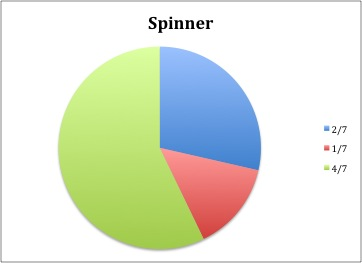
\includegraphics[scale=.6]{ReviewSpinner}\end{center}
\end{multicols}
\begin{solution} This is the same problem as Exercise~\ref{Spinner}
with $E$ the event that the spinner lands on a primary
color and $F$ the event that the spinner lands on an ISU color.
\end{solution}

\question You roll two regular six-sided dice. Calculate the probability
that the sum of the numbers showing is greater than 9 given that
the first die shows 5.
\begin{solution} The sum will be greater than 9 if the second die
shows 5 or 6.
This will occur with probability $\frac{2}{6}=\frac{1}{3}$.
\end{solution}

\question The National Vital Statistics Report estimates
that a US resident will live at least 80~years with probability~$.091$
and at least 90~years with probability~$0.047$.
What is the probability that a resident lives at least 90~years
given that he or she is now 80~years old?
\begin{solution}
Let $E$ be the event that the resident lives at least 80~years
and $F$ the event that the resident lives at least 90~years.
Note that $E\cap F=F$. Thus
\[P\left(F\mid E\right)
=\frac{P\left(F\cap E\right)}{P\left(E\right)}
=\frac{P\left(F\right)}{P\left(E\right)}
=\frac{0.047}{0.091}\approx 0.516.\]
\end{solution}

\uplevel{\bf Permutations.}
\question In a swimming race involving eight swimmers, only the three
with the fastest times are observed,
namely, first, second, third places.
How many possible outcomes of the race are there?
\begin{solution} $8\cdot 7\cdot 6=336$ \end{solution}

\question I have five cars, but only a two-stall garage, so I
park three of my cars on the street. 
The stall closest to the house is the most useful stall since
it has a garage door opener. In how many
ways can I park my cars in the garage?
\begin{solution}$5\cdot 4=20$\end{solution}

\question Five children arrive at my house on Halloween,
but I only have three pieces of fruit remaining to distribute, namely
a banana, a pear, and an apple. In how many ways can I distribute
fruit to the children?
\begin{solution} $5\cdot 4\cdot 3=60$\end{solution}

\uplevel{\bf Combinations, binomial coefficients, number of subsets.}
\question
\begin{parts}
\part How many subsets of a set of size eight are there?
\part A {\em byte} is a sequence of eight {\em bits}, each
of which representing either zero or one. How many bytes are possible?
\part If a pizza restaurant offers eight different toppings
for customers to choose among, how many ways to order a pizza are there?
\end{parts}
\begin{solution} $2^8=256$ is the answer to all three questions.\end{solution}

\question How many four-person subcommittees can be formed
from a committee of ten people under the following circumstances?
\begin{parts}
\part There are no restrictions.
\part Alice and Quinn must both be on the subcommittee.
\part Either Alice or Quinn (but not both) must be on the subcommittee.
\end{parts}
\begin{solution}
If there are no restrictions this can
be done in $\ncr{10}{4}=210$ ways.
However, if both Alice and Quinn must be on the subcommittee
then there are $\ncr{8}{2}=28$ possibilities since the two remaining
members of the subcommittee
must be selected from among the eight remaining members of the committee.
If Alice or Quinn but not both must be on the subcommittee,
then there are $2\cdot\ncr{8}{3}=112$ possibilities.
This is because either Alice or Quinn must be selected,
after which the three remaining members of the subcommittee
must be selected from among the eight remaining members of the committee.
\end{solution}

\question How many five-card poker hands have all picture cards?
\begin{solution}$\ncr{12}{5}=792$\end{solution}

\uplevel{\bf Definitions of all the poker hands.}

\uplevel{\bf Problems involving improving poker hands by exchanging cards.}
\question Playing poker, your receive the cards
$2\diamondsuit,4\clubsuit,5\diamondsuit,5\spadesuit,10\diamondsuit$.
If you exchange $4\clubsuit,5\spadesuit$ for two new cards,
then what is the probability that the new hand will be a flush?
\begin{solution}
Since you hold three diamonds, there remain ten in the deck.
Two of them could be dealt to you in $\ncr{10}{2}=45$ ways.
Now since $47$~cards remain, any two cards could be dealt to you in
$\ncr{47}{2}=1081$ ways. So your probability of completing your flush
is $\frac{45}{1081}\approx 0.0416$.
\end{solution}

\question Playing poker, your receive the cards
$2\diamondsuit,4\clubsuit,5\diamondsuit,5\spadesuit,10\diamondsuit$.
If you exchange $2\diamondsuit,4\clubsuit,10\diamondsuit$ for
three new cards, then what is the probability that the new hand
will have three-of-a-kind?
\begin{solution}
There remain two cards of rank five in the deck. There are two
ways to choose one of them, and $\ncr{45}{2}=990$ ways to choose
two other cards of rank other than five. Now since any three cards
can be dealt to you in $\ncr{47}{3}=16,215$ ways, your probability
of receiving exactly one five is $\frac{2\cdot 990}{16215}\approx 0.1221$.
\end{solution}
\uplevel{\bf Binomial probability.}
\question If a baseball player has a batting average
of $0.350$ then what is the probability that he
will hit the ball the following number of times in his next four
times at bat?
\begin{parts}
\part Exactly twice
\begin{solution}
$\ncr{4}{2}\left(0.35\right)^2\left(0.65\right)^2\approx 0.311$
\end{solution}
\part At least twice
\begin{solution}
$\ncr{4}{2}\left(0.35\right)^2\left(0.65\right)^2
+\ncr{4}{3}\left(0.35\right)^3\left(0.65\right)^1
+\ncr{4}{4}\left(0.35\right)^4\left(0.65\right)^0\approx 0.568$
\end{solution}
\end{parts}

\question If $60\%$ of the electorate supports the mayor
then what is the probability that in a random sample
of 10~voters, fewer than half support her?
\begin{solution} Since $60\%$ of the electorate support the mayor,
the probability that a randomly selected voter supports her
is $p=0.6$. So the probability that exactly $r$ of the ten randomly
selected voters
supports her is $\ncr{10}{r}\left(0.6\right)^r\left(0.4\right)^{10-r}$.
Repeating this calculation for $r=0,1,2,3,4$ and adding gives
\begin{multline*}
\ncr{10}{0}\left(0.6\right)^0\left(0.4\right)^{10}
+\ncr{10}{1}\left(0.6\right)^1\left(0.4\right)^9
+\ncr{10}{2}\left(0.6\right)^2\left(0.4\right)^8\\
+\ncr{10}{3}\left(0.6\right)^3\left(0.4\right)^7
+\ncr{10}{4}\left(0.6\right)^4\left(0.4\right)^6
\approx 0.1662.
\end{multline*}
\end{solution}

\uplevel{\bf Blackjack.}
\question Playing blackjack with the dealer dealing
from several decks, you receive the cards $K\spadesuit,6\heartsuit$
initially.
\begin{parts}
\part What is the probability that you won't bust if you take another card?
\begin{solution} We assume that the probability of receiving a card
of a particular rank is $\frac{1}{13}$ since several decks of cards are
being used. Thus the ranks that won't bust you are
$A,2,3,4,5$ so $\frac{5}{13}$ is the probability that you won't bust.
\end{solution}
\part Suppose you request another card and receive $2\clubsuit$.
What is the probability that you won't bust if you take another card?
\begin{solution} Now your sum is 18, so the ranks that won't bust
you are $A,2,3$. Thus the probability that you won't bust
is $\frac{3}{13}$.
\end{solution}
\end{parts}
\end{questions}
\end{document}
